% !TeX root = Protokoll.tex
\subsection{Methode zur Kristallstrukturbestimmung}
\begin{figure}[h!]
	\centering
	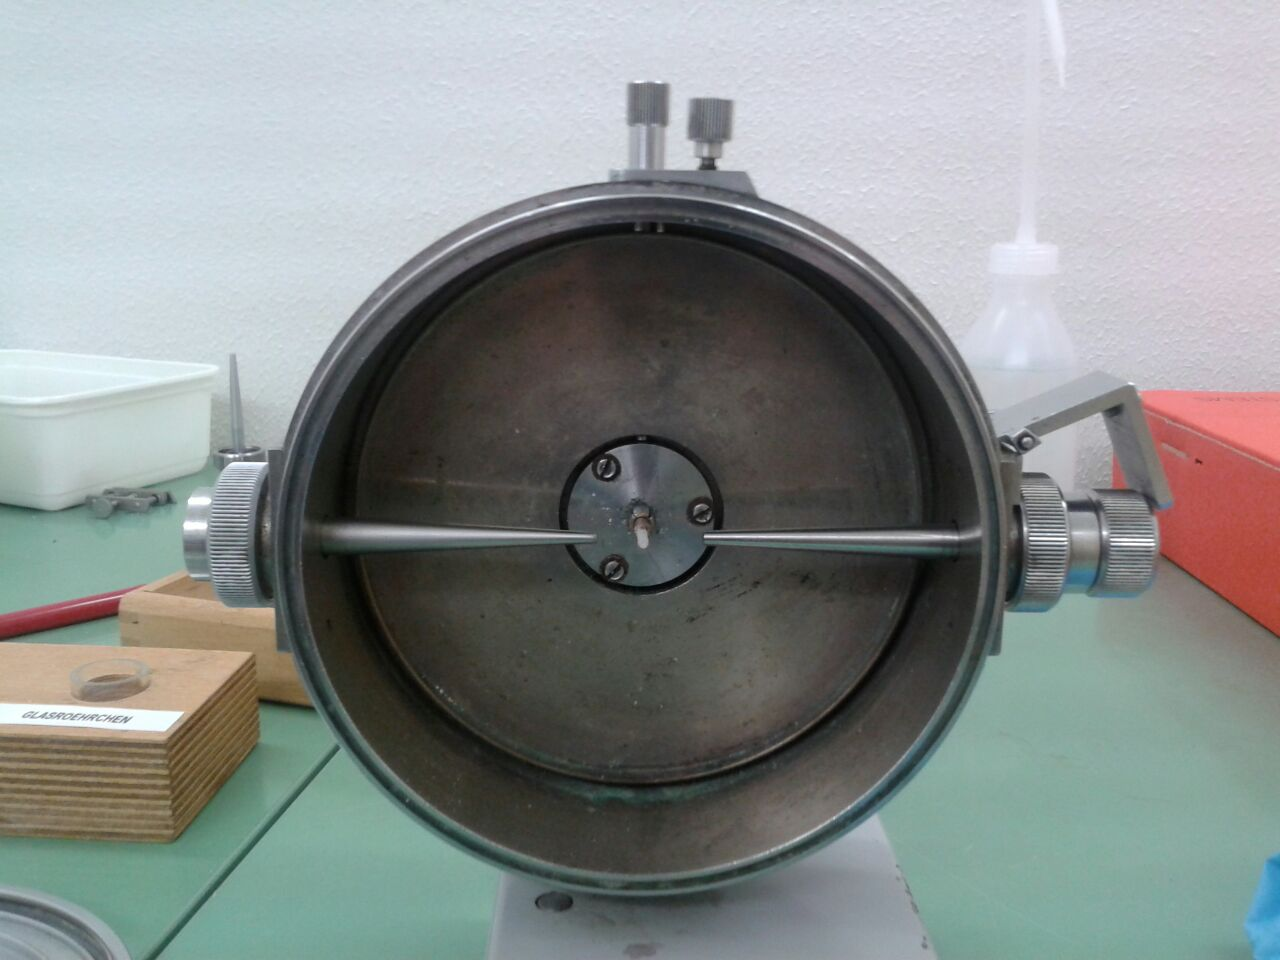
\includegraphics[scale = 0.25]{../Grafiken/Aufbau.jpg}
	\caption{Aufbau zur Erstellung einer Debye-Scherrer-Aufnahme.}\label{fig:Aufbau}
\end{figure}
Das Ziel der Kristallstrukturbestimmung ist die Größe, die Form und die Anordnung der Atome innerhalb der Elementarzelle.\\ 
In \cref{fig:Aufbau} ist der verwendete Aufbau zu sehen. Die Beiden Nadeln sind hohl und sind Führungen für die Röntgenstrahlen. Die Rechte Nadel ist verschlossen damit keine Röntgenstrahlen austreten können. In der Mitte ist die Probe zusehen, dabei wird die Probe auf ein Glasröhrchen in pulverisiertet Form aufgebracht. Die Kristalle verlieren durch das pulverisieren nicht die Eigenschaften, zudem sind die Ausrichtung der Kristalle über alle Raumwinkel verteilt, dies sorgt dafür das mit hoher Wahrscheinlichkeit Reflexe auftreten. Die Probe muss mithilfe der Justierschraube auf die Optische Achse eingestellt werden. Die Probe wird mithilfe eines Motors gedreht damit die Auftretenden Reflexe gleichmäßig sind, dies muss auch bei der Justage beachtet werden.\\
In der außen wand des Zylinders wird ein Film eingespannt, auf ihm werden nach dem Bestrahlen der Probe Ringe zusehen sein, deren Radien proportional zu dem Beugungswinkel sind. Der Film muss unter Rotlicht eingespannt werden und darf nicht mit bloßen Händen berührt werden. Der Zylinder kann dann Verschlossen werden.
Danach kann der Zylinder in die Apparatur eingebaut werden in der die Probe bestrahlt werden kann.
Nach dem Bestrahlen muss der Film nur noch entwickelt werden, was ebenfalls unter Rotlicht passieren muss.
\begin{figure}[h!]
	\centering
	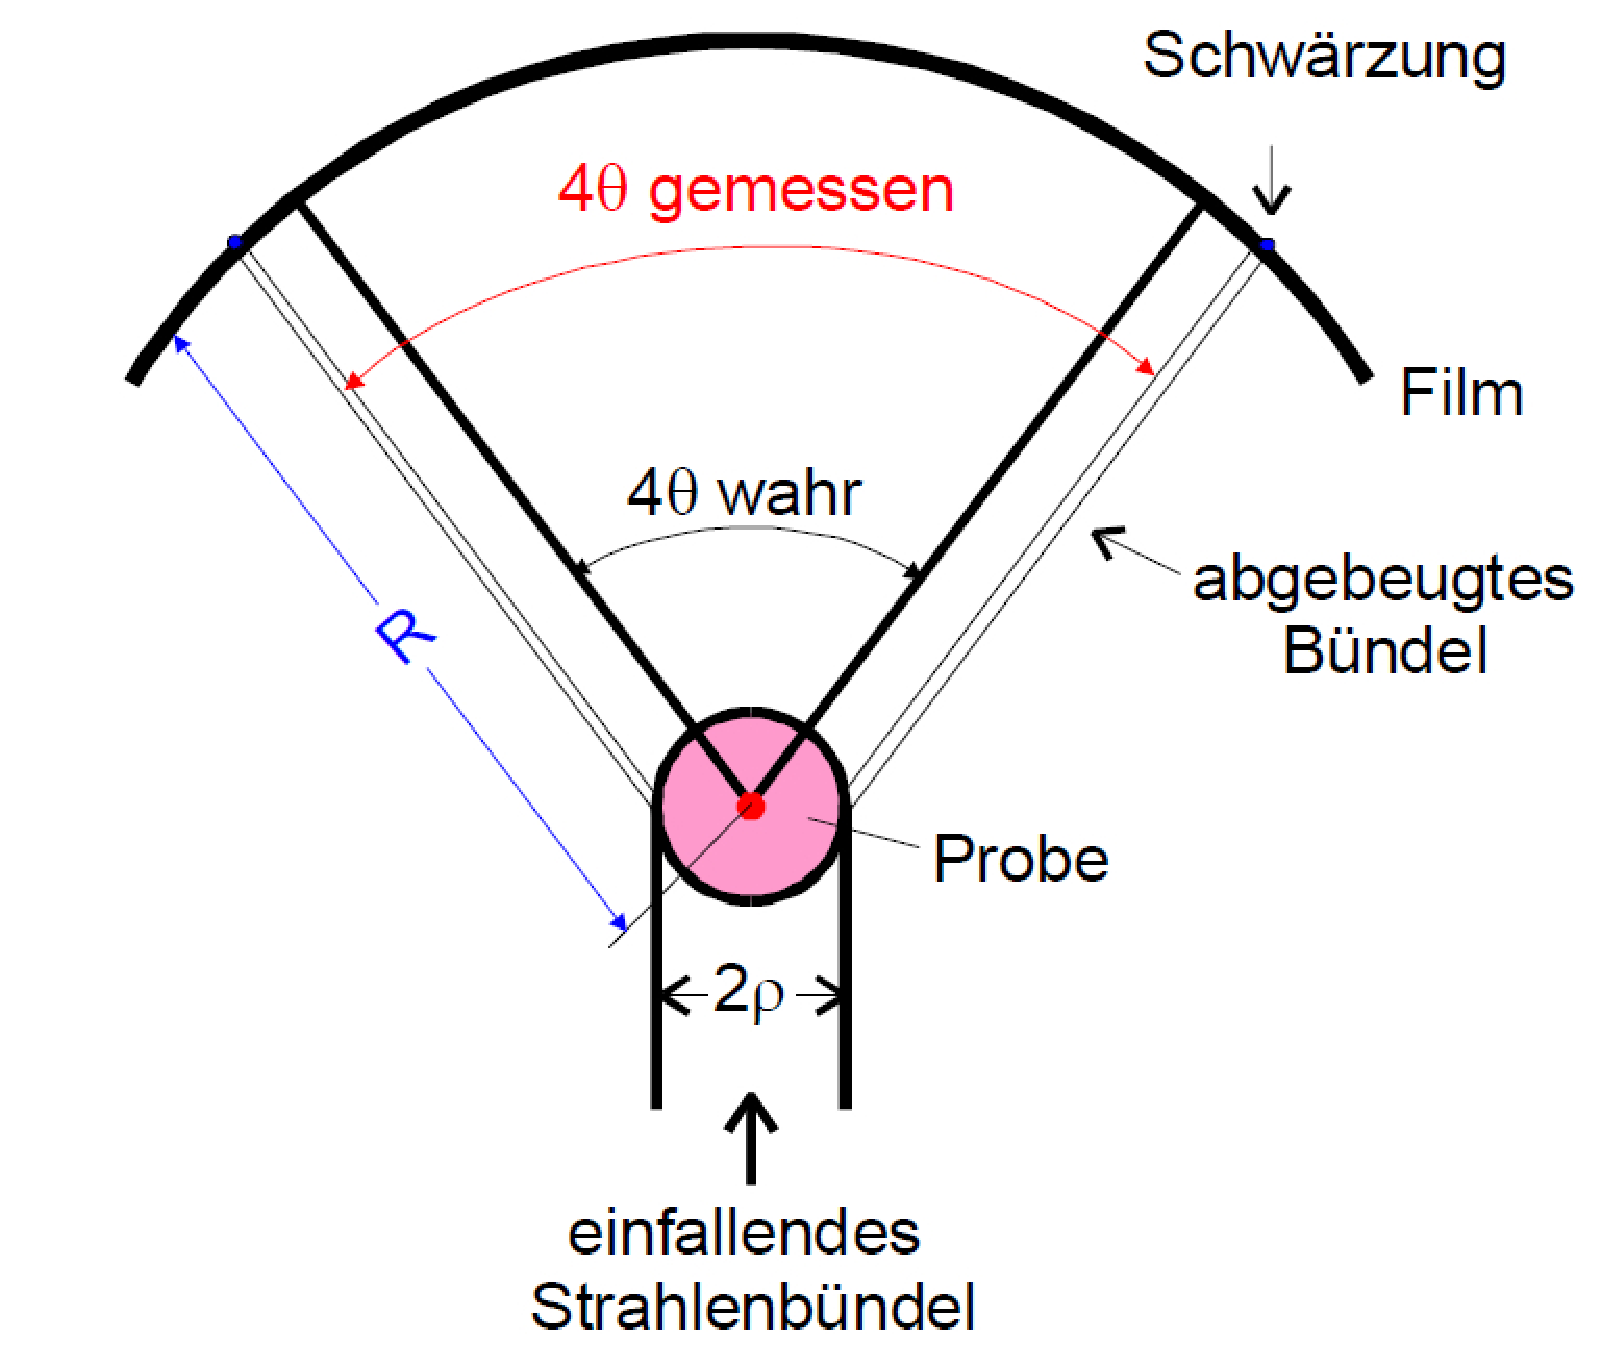
\includegraphics[scale=0.4]{../Grafiken/ErsteKorrektur.pdf}
	\caption{Schema zur Verdeutlichung der Korrektur, die durch Beugung am Zylindermantel der Probe entsteht\cite{V41}.}
\end{figure}
Bei diesem Aufbau treten zwei Systematische Fehler auf. Der erste ist das die Probe fast alle einfallenden Röntgenstrahlen absorbiert. Das bedeutet es wird nur an einem schmalen Streifen des Zylindermantels gebeugt. Das sorgt dafür das 4$\theta$ zu groß gemessen wird. An die Gitterkonstante muss folgende Korrektur angebracht werden um das zu berücksichtigen.
\begin{align}
	\frac{\Delta a_A}{a}=\frac{\rho}{2R}\left(1-\frac{R}{F}\right)\frac{\cos^2\theta}{\theta}
\end{align}
Dabei ist $\rho$ der Probenradius und $R$ der Kammerradius der 57,4mm beträgt und $F$ der Abstand vom Fokus zur Probe der 130mm beträgt.\\
\begin{figure}[h!]
	\centering
	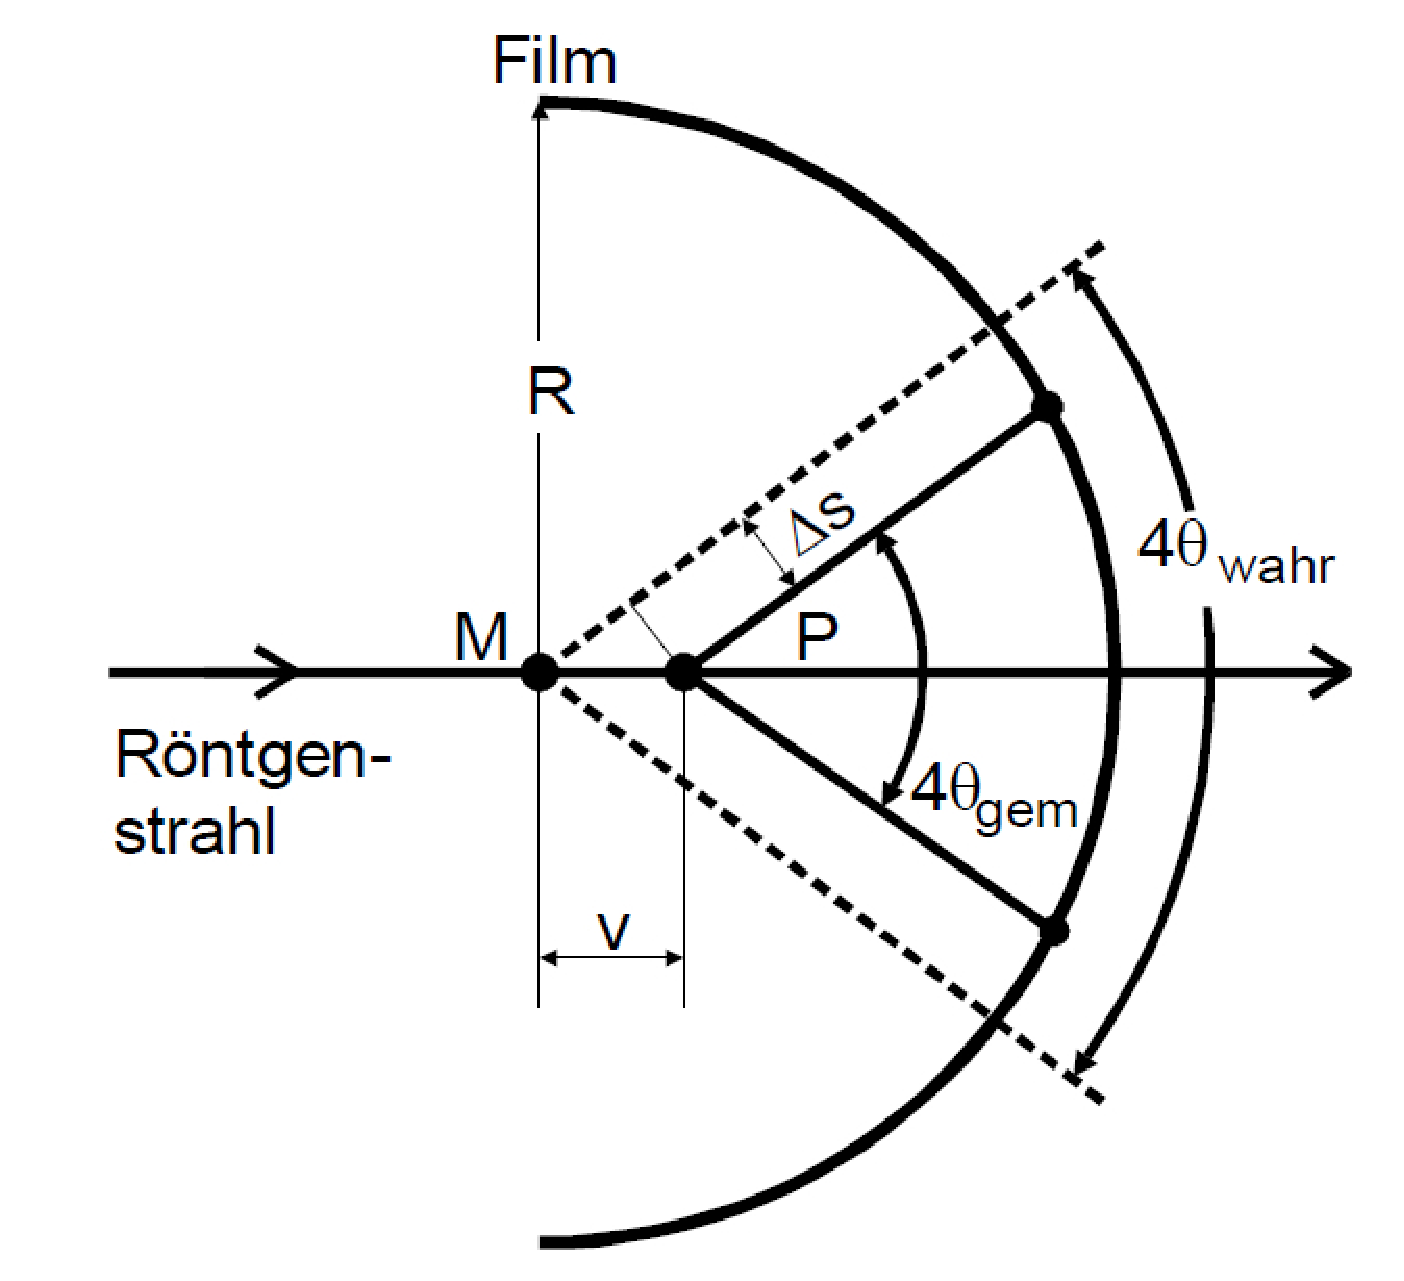
\includegraphics[scale=0.4]{../Grafiken/ZweiteKorrektur.pdf}
	\caption{Veranschaulichung der zweiten Korrektur, die durch Verschiebung der Probe von dem Mittelpunkt des Zylinders entsteht.\cite{V41}}\label{fig:ZweiteKorrektur}
\end{figure}
Der zweite systematische Fehler entsteht dadurch, dass sich die Probe nicht Genau in der Mitte des Filmszylinders ist. Die Korrektur ist dann
\begin{align}
	\frac{\Delta a_V}{a}=\frac{v}{R}\cos^2\theta,
\end{align}
mit $v$ dem Abstand nach \cref{fig:ZweiteKorrektur}. Weil die Korrektur von $\Delta a_A$ viel kleiner als die von $\Delta a_V$ ist wird 
\begin{align}
	\Delta a_\text{g}=\Delta a_A+ \Delta a_V \propto \cos^2\theta
\end{align}
betrachtet, wobei $\Delta a_\text{g}$ die gesamte Korrektur ist.